% Template for a Computer Science Tripos Part II project dissertation
\documentclass[12pt,a4paper,twoside,openright]{report}
\usepackage[pdfborder={0 0 0}]{hyperref}    % turns references into hyperlinks
\usepackage[margin=25mm]{geometry}  % adjusts page layout
\usepackage{graphicx}  % allows inclusion of PDF, PNG and JPG images
\usepackage{verbatim}
\usepackage{docmute}   % only needed to allow inclusion of proposal.tex

\raggedbottom                           % try to avoid widows and orphans
\sloppy
\clubpenalty1000%
\widowpenalty1000%

\renewcommand{\baselinestretch}{1.1}    % adjust line spacing to make
                                        % more readable

\begin{document}

\bibliographystyle{plain}


%%%%%%%%%%%%%%%%%%%%%%%%%%%%%%%%%%%%%%%%%%%%%%%%%%%%%%%%%%%%%%%%%%%%%%%%
% Title


\pagestyle{empty}

\rightline{\LARGE \textbf{Henry Mattinson}}

\vspace*{60mm}
\begin{center}
\Huge
\textbf{Excello: End-user music programming in Excel} \\[5mm]
Computer Science Tripos -- Part II \\[5mm]
Christ's College \\[5mm]
\today  % today's date
\end{center}

%%%%%%%%%%%%%%%%%%%%%%%%%%%%%%%%%%%%%%%%%%%%%%%%%%%%%%%%%%%%%%%%%%%%%%%%%%%%%%
% Proforma, table of contents and list of figures

\pagestyle{plain}

\chapter*{Proforma}

{\large
\begin{tabular}{ll}
Name:               & \bf Henry Mattinson                      \\
College:            & \bf Christ's College                     \\
Project Title:      & \bf Excello: End-user music programming in Excel \\
Examination:        & \bf Computer Science Tripos -- Part II, June 2019  \\
Word Count:         & \bf ????\footnotemark[1]  \\
Project Originator: & Alan Blackwell                    \\
Supervisor:         & Dr Advait Sarkar                    \\
\end{tabular}
}
\footnotetext[1]{This word count was computed
by \texttt{detex diss.tex | tr -cd '0-9A-Za-z $\tt\backslash$n' | wc -w}
}
\stepcounter{footnote}


\section*{Original Aims of the Project}

The main aim of the project was to create a system for music expression and playback allowing users to play individual notes and chords and define their durations, define multiple parts, play loops, define sequences of notes and chords and be able to call these for playback and define the tempo of playback. Followed by the implementation of a converter from an existing musical notation to the Excel system (with compression as an extension) and usability testing of the Excel system.

\section*{Work Completed}

I designed a notation for music expression in Excel and built a prototype (Excello) satisfying the success criteria above. Participatory design sessions with 21 users served as formative evaluation leading to the implementation of many additional features as extensions. I contributed part of my implementation to an open-source library, this has been merged and published. I built a converter from MIDI to the Excello notation which can convert exactly or perform lossy compression. This was used to translate a corpus of music to the Excello notation. I performed summative evaluation with the users from the participatory design.

\section*{Special Difficulties}

None.

\newpage
\section*{Declaration}

I, Henry Mattinson of Christ's College, being a candidate for Part II of the Computer
Science Tripos, hereby declare
that this dissertation and the work described in it are my own work,
unaided except as may be specified below, and that the dissertation
does not contain material that has already been used to any substantial
extent for a comparable purpose.

\bigskip
\leftline{Signed [signature]}

\medskip
\leftline{Date [date]]}

\tableofcontents

% \listoffigures

% \newpage
% \section*{Acknowledgements}
%
% This document owes much to an earlier version written by Simon Moore
% \cite{Moore95}.  His help, encouragement and advice was greatly
% appreciated.

%%%%%%%%%%%%%%%%%%%%%%%%%%%%%%%%%%%%%%%%%%%%%%%%%%%%%%%%%%%%%%%%%%%%%%%
% now for the chapters

\pagestyle{headings}

\chapter{Introduction}

\section{Overview of the files}

This document consists of the following files:

\begin{itemize}
\item \texttt{makefile} --- The makefile for the dissertation and
                         Project Proposal
\item \texttt{diss.tex} --- The dissertation
\item \texttt{proposal.tex}  --- The project proposal
\item \texttt{figs} -- A directory containing diagrams and pictures
\item \texttt{refs.bib} --- The bibliography database
\end{itemize}
\section{Building the document}

This document was produced using \LaTeXe which is based upon
\LaTeX\cite{Lamport86}.  To build the document you first need to
generate \texttt{diss.aux} which, amongst other things, contains the
references used.  This if done by executing the command:

\texttt{pdflatex diss}

\noindent
Then the bibliography can be generated from \texttt{refs.bib} using:

\texttt{bibtex diss}

\noindent
Finally, to ensure all the page numbering is correct run \texttt{pdflatex}
on \texttt{diss.tex} until the \texttt{.aux} files do not change.  This
usually takes 2 more runs.

\subsection{The makefile}

To simplify the calls to \texttt{pdflatex} and \texttt{bibtex},
a makefile has been provided, see Appendix~\ref{makefile}.
It provides the following facilities:

\begin{description}

\item\texttt{make} \\
 Display help information.

\item\texttt{make proposal.pdf} \\
 Format the proposal document as a PDF.

\item\texttt{make view-proposal} \\
 Run \texttt{make proposal.pdf} and then display it with a Linux PDF viewer
 (preferably ``okular'', if that is not available fall back to ``evince'').

\item\texttt{make diss.pdf} \\
 Format the dissertation document as a PDF.

\item\texttt{make count} \\
Display an estimate of the word count.

\item\texttt{make all} \\
Construct \texttt{proposal.pdf} and \texttt{diss.pdf}.

\item\texttt{make pub} \\ Make \texttt{diss.pdf}
and place it in my \texttt{public\_html} directory.

\item\texttt{make clean} \\ Delete all intermediate files except the
source files and the resulting PDFs. All these deleted files can
be reconstructed by typing \texttt{make all}.

\end{description}


\section{Counting words}

An approximate word count of the body of the dissertation may be
obtained using:

\texttt{wc diss.tex}

\noindent
Alternatively, try something like:

\verb/detex diss.tex | tr -cd '0-9A-Z a-z\n' | wc -w/


\chapter{Preparation}

This chapter is empty!


\chapter{Implementation}

\section{Verbatim text}

Verbatim text can be included using \verb|\begin{verbatim}| and
\verb|\end{verbatim}|. I normally use a slightly smaller font and
often squeeze the lines a little closer together, as in:

{\renewcommand{\baselinestretch}{0.8}\small
\begin{verbatim}
GET "libhdr"

GLOBAL { count:200; all  }

LET try(ld, row, rd) BE TEST row=all
                        THEN count := count + 1
                        ELSE { LET poss = all & ~(ld | row | rd)
                               UNTIL poss=0 DO
                               { LET p = poss & -poss
                                 poss := poss - p
                                 try(ld+p << 1, row+p, rd+p >> 1)
                               }
                             }
LET start() = VALOF
{ all := 1
  FOR i = 1 TO 12 DO
  { count := 0
    try(0, 0, 0)
    writef("Number of solutions to %i2-queens is %i5*n", i, count)
    all := 2*all + 1
  }
  RESULTIS 0
}
\end{verbatim}
}

\section{Tables}

\begin{samepage}
Here is a simple example\footnote{A footnote} of a table.

\begin{center}
\begin{tabular}{l|c|r}
Left      & Centred & Right \\
Justified &         & Justified \\[3mm]
%\hline\\%[-2mm]
First     & A       & XXX \\
Second    & AA      & XX  \\
Last      & AAA     & X   \\
\end{tabular}
\end{center}

\noindent
There is another example table in the proforma.
\end{samepage}

\section{Simple diagrams}

Simple diagrams can be written directly in \LaTeX.  For example, see
figure~\ref{latexpic1} on page~\pageref{latexpic1} and see
figure~\ref{latexpic2} on page~\pageref{latexpic2}.

\begin{figure}
\setlength{\unitlength}{1mm}
\begin{center}
\begin{picture}(125,100)
\put(0,80){\framebox(50,10){AAA}}
\put(0,60){\framebox(50,10){BBB}}
\put(0,40){\framebox(50,10){CCC}}
\put(0,20){\framebox(50,10){DDD}}
\put(0,00){\framebox(50,10){EEE}}

\put(75,80){\framebox(50,10){XXX}}
\put(75,60){\framebox(50,10){YYY}}
\put(75,40){\framebox(50,10){ZZZ}}

\put(25,80){\vector(0,-1){10}}
\put(25,60){\vector(0,-1){10}}
\put(25,50){\vector(0,1){10}}
\put(25,40){\vector(0,-1){10}}
\put(25,20){\vector(0,-1){10}}

\put(100,80){\vector(0,-1){10}}
\put(100,70){\vector(0,1){10}}
\put(100,60){\vector(0,-1){10}}
\put(100,50){\vector(0,1){10}}

\put(50,65){\vector(1,0){25}}
\put(75,65){\vector(-1,0){25}}
\end{picture}
\end{center}
\caption{A picture composed of boxes and vectors.}
\label{latexpic1}
\end{figure}

\begin{figure}
\setlength{\unitlength}{1mm}
\begin{center}

\begin{picture}(100,70)
\put(47,65){\circle{10}}
\put(45,64){abc}

\put(37,45){\circle{10}}
\put(37,51){\line(1,1){7}}
\put(35,44){def}

\put(57,25){\circle{10}}
\put(57,31){\line(-1,3){9}}
\put(57,31){\line(-3,2){15}}
\put(55,24){ghi}

\put(32,0){\framebox(10,10){A}}
\put(52,0){\framebox(10,10){B}}
\put(37,12){\line(0,1){26}}
\put(37,12){\line(2,1){15}}
\put(57,12){\line(0,2){6}}
\end{picture}

\end{center}
\caption{A diagram composed of circles, lines and boxes.}
\label{latexpic2}
\end{figure}



\section{Adding more complicated graphics}

The use of \LaTeX\ format can be tedious and it is often better to use
encapsulated postscript (EPS) or PDF to represent complicated graphics.
Figure~\ref{epsfig} and~\ref{xfig} on page \pageref{xfig} are
examples. The second figure was drawn using \texttt{xfig} and exported in
{\tt.eps} format. This is my recommended way of drawing all diagrams.


\begin{figure}[tbh]
\centerline{
\includegraphics{figs/cuarms.pdf}}
\caption{Example figure using encapsulated postscript}
\label{epsfig}
\end{figure}

\begin{figure}[tbh]
\vspace{4in}
\caption{Example figure where a picture can be pasted in}
\label{pastedfig}
\end{figure}


\begin{figure}[tbh]
\centerline{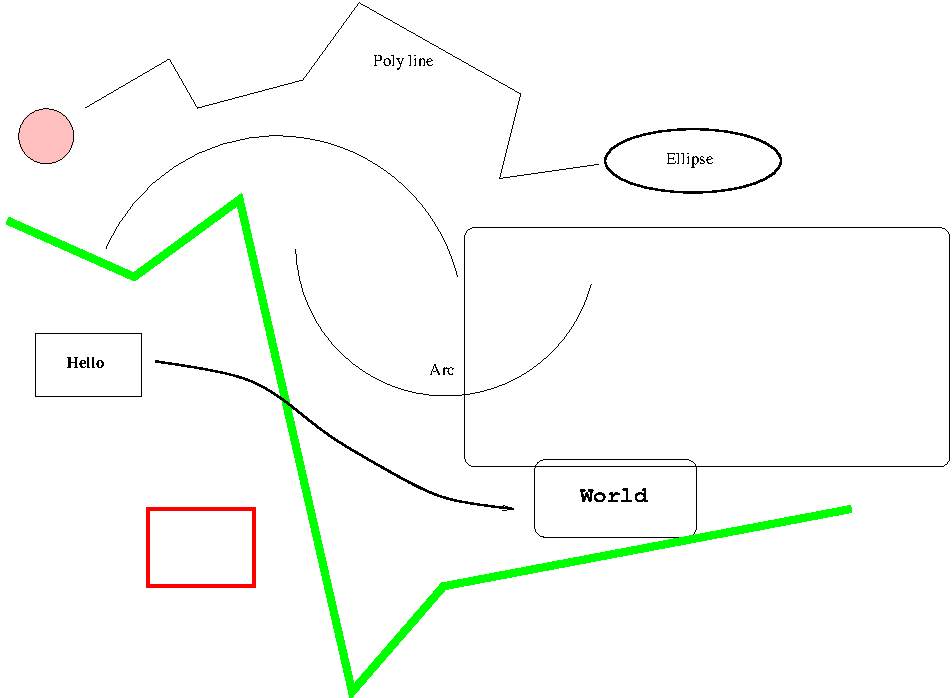
\includegraphics{figs/diagram.pdf}}
\caption{Example diagram drawn using \texttt{xfig}}
\label{xfig}
\end{figure}


\chapter{Evaluation}

\section{Printing and binding}

Use a ``duplex'' laser printer that can print on both sides to print
two copies of your dissertation. Then bind them, for example using the
comb binder in the Computer Laboratory Library.

\section{Further information}

See the Unix Tools notes at

\url{http://www.cl.cam.ac.uk/teaching/current-1/UnixTools/materials.html}


\chapter{Conclusion}

I hope that this rough guide to writing a dissertation is \LaTeX\ has
been helpful and saved you time.


%%%%%%%%%%%%%%%%%%%%%%%%%%%%%%%%%%%%%%%%%%%%%%%%%%%%%%%%%%%%%%%%%%%%%
% the bibliography
\addcontentsline{toc}{chapter}{Bibliography}
\bibliography{refs}

%%%%%%%%%%%%%%%%%%%%%%%%%%%%%%%%%%%%%%%%%%%%%%%%%%%%%%%%%%%%%%%%%%%%%
% the appendices
\appendix

\chapter{Latex source}

\section{diss.tex}
{\scriptsize\verbatiminput{diss.tex}}

\section{proposal.tex}
{\scriptsize\verbatiminput{proposal.tex}}

\chapter{Makefile}

\section{makefile}\label{makefile}
{\scriptsize\verbatiminput{makefile.txt}}

\section{refs.bib}
{\scriptsize\verbatiminput{refs.bib}}


\chapter{Project Proposal}

\documentclass[]{article}
\usepackage{lmodern}
\usepackage{amssymb,amsmath}
\usepackage{ifxetex,ifluatex}
\usepackage{fixltx2e} % provides \textsubscript
\ifnum 0\ifxetex 1\fi\ifluatex 1\fi=0 % if pdftex
  \usepackage[T1]{fontenc}
  \usepackage[utf8]{inputenc}
\else % if luatex or xelatex
  \ifxetex
    \usepackage{mathspec}
  \else
    \usepackage{fontspec}
  \fi
  \defaultfontfeatures{Ligatures=TeX,Scale=MatchLowercase}
\fi
% use upquote if available, for straight quotes in verbatim environments
\IfFileExists{upquote.sty}{\usepackage{upquote}}{}
% use microtype if available
\IfFileExists{microtype.sty}{%
\usepackage[]{microtype}
\UseMicrotypeSet[protrusion]{basicmath} % disable protrusion for tt fonts
}{}
\PassOptionsToPackage{hyphens}{url} % url is loaded by hyperref
\usepackage[unicode=true]{hyperref}
\hypersetup{
            pdfborder={0 0 0},
            breaklinks=true}
\urlstyle{same}  % don't use monospace font for urls
\IfFileExists{parskip.sty}{%
\usepackage{parskip}
}{% else
\setlength{\parindent}{0pt}
\setlength{\parskip}{6pt plus 2pt minus 1pt}
}
\setlength{\emergencystretch}{3em}  % prevent overfull lines
\providecommand{\tightlist}{%
  \setlength{\itemsep}{0pt}\setlength{\parskip}{0pt}}
\setcounter{secnumdepth}{0}
% Redefines (sub)paragraphs to behave more like sections
\ifx\paragraph\undefined\else
\let\oldparagraph\paragraph
\renewcommand{\paragraph}[1]{\oldparagraph{#1}\mbox{}}
\fi
\ifx\subparagraph\undefined\else
\let\oldsubparagraph\subparagraph
\renewcommand{\subparagraph}[1]{\oldsubparagraph{#1}\mbox{}}
\fi

% set default figure placement to htbp
\makeatletter
\def\fps@figure{htbp}
\makeatother


\date{}

\begin{document}

\section{Music Generation in Microsoft Excel}\label{header-n3}

\subsection{Introduction}\label{header-n6}

Excel and other spreadsheet tools have become universally popular, both
in businesses and individually, for storing, processing and visualising
data. However, at present there is not the functionality for the
playback of music. Many existing music production packages utilise a
grid like format with time passing along the x-axis and parts down the
y-axis. Therefore, spreadsheets seem like a promising environment from
which to be able to carry out basic music composition in this format and
others.

Many people are already familiar with representing concepts in
spreadsheet form. This project will explore the use of Excel for musical
expression and, as an extension, as a live music coding environment.

\subsection{Starting Point}\label{header-n9}

No existing work or further knowledge than part Ia and Ib courses. I am
a seasoned musician and musical theory enthusiast so possess all the
required musical theory knowledge.

I will be building on top of existing spreadsheet service. I would aim
to use the Microsoft Office API Office.JS (a public API) and use Add-ins
for adding my own functionality, if there is sufficient support for
sound. This is publicly available. If not, I would either be able to use
a Typescript prototype of Excel from Microsoft or an existing open
source JavaScript implementation of a spreadsheet.

\subsection{Substance and Structure}\label{header-n12}

By using a TypeScript or JavaScript version of Excel run in browser,
playback functionality can be built on top of the web audio API.
Functionality for note and sequence synthesis functions will be
required. A converter from an existing formal music specification to the
spreadsheet representation will be implemented. As an extension, live
coding can be implemented.

Firstly I will have to establish what notation is used within the cells.
Within a given cell, I would like to be able to play single notes and
chords. Beyond this defining scales and arpeggios would be useful for
reducing the size of grid required to define pieces. This notation must
then be interpreted with a resulting call to the browser audio API. It
would also be desirable to be able to define sequences of notes (e.g.
baselines, repeating melodies) elsewhere in the grid and then be able to
call these elsewhere in the playback. This means that users do not have
to copy and paste repeating sections and it would also be clearer where
sections are repeated.

Next, the representation that is supported between cells must be decided
and implemented. The flexibility of spreadsheets allows users to define
their own secondary notation in the way that sections within the grid
are laid out. As a result, allowing for the relative positions of
different sections within a sheet and their orientation to vary would
allow familiar Excel users to continue defining their own layout. The
definition and re-use of phrases and parts would allow for fast
prototyping of musical ideas. The representation will likely be that of
a main playback loop (which can be split into multiple parts), with
definitions of sequences outside of this main loop section.

After establishing my notation and supported layouts, the program must
compile this representation into audio output for playback. Firstly,
defined variables (e.g. Tempo) and regions where melodic lines are
defined out of the main playback loop must be detected. Next, the main
playback loop region and its orientation must be detected. After this,
the information can be processed and converted into calls to the audio
API.

As an extension, I can add support for live music coding. To facilitate
live music coding, it should be possible to change notes within the grid
and recompile whilst playback is occurring. Live music coding encourages
a loop based approach to music so run/compiled changes to the grid
should become apparent in the playback whilst not requiring a restart of
the output. The program would be able to parse the data within the
spreadsheet and identify different regions and declarations. From this
it would convert the main playback loop with the output being calls to
the growers audio API. This would include integrating sequences that are
defined out of the main loop but called with in.

Once the representation of musical structure has been decided and the
playback of this representation implemented, I will implement a
conversion from some form of formal music notation (e.g. MusicXML or
MIDI) to the spreadsheet representation. Existing pieces can then be
immediately transformed into the spreadsheet layout and played back
using the spreadsheet music API.

As an extension I could explore reducing the size of the representation
within the spreadsheet. For example, a repeated chord sequence could
only be shown once in the spreadsheet whilst keeping an understandable
representation. Whilst this is not conventional compression, similar
lossless or lossy algorithms for eliminating statistical redundancy can
be employed.

The project has the following main sections:

\begin{enumerate}
\def\labelenumi{\arabic{enumi}.}
\item
  Facilitating audio playback from a spreadsheet, run from the browser.
\item
  Execution and playback of musical definition code in the grid cells.
\item
  Playback of multiple cells where time is represented in an axis or the
  code within cells.
\item
  Implementation of a converter from a formal music notation to the
  spreadsheet representation.
\item
  Evaluation and the preparation of examples to demonstrate the success
  of the implementation.
\item
  User testing.
\item
  Writing the dissertation.
\end{enumerate}

\subsection{Evaluation and Success Criteria}\label{header-n37}

A successful implementation should allow a user to carry out the
following:

\begin{itemize}
\item
  Play individual notes and chords and define their durations.
\item
  Defining multiple parts.
\item
  Play loops.
\item
  Define sequences of notes and chords and be able to call these for
  playback.
\item
  Define the tempo of playback.
\end{itemize}

Qualitatively, use of the music playback API can be analysed using a
friction analysis approach as in {[}3{]} and a cognitive dimensions
profile strategy.

With some basic explanation, users can be measured carrying out simple
tasks or free composition. From this we can measure Time To Hello World
(TTHW) (e.g. playing a note). Friction diagrams generated based on
observation of a user working with the program in a usability study can
be used to evaluate the productivity of users of the tool.

We define the following desirable features in a cognitive dimensions
profile. This defines the desirable structural usability properties of
the API and interaction UI.

\begin{itemize}
\item
  Reasonable \textbf{closeness of mapping} (use of the grid structure
  should allow for much higher closeness of mapping than e.g. Sonic Pi
  where there is only one file of code).
\item
  High \textbf{consistency} for the definition of notes and chords
  within phrases.
\item
  Layout within the grid should allow for high \textbf{secondary
  notation}
\item
  Low \textbf{viscosity}
\item
  High \textbf{visibility}
\end{itemize}

We shall then use a Cognitive Dimensions questionnaire to empirically
categorise users' response to it. Evaluation can be carried out by
comparing that response to this desired profile.

Quantitatively, the expressiveness of the API can be verified by a
translation of a musical corpus from the formal notation to the
spreadsheet representation.

The compression rates achieved in the compression of the representation
can also be measured and compared to a benchmark of a naive conversion.

\paragraph{Success criteria}\label{header-n67}

For the project to be deemed a success the following must be completed:

\begin{itemize}
\item
  Implementation of an API for music playback within a spreadsheet using
  the above implementation features.
\item
  Implementation of a converter from formal music notation to the
  spreadsheet representation.
\item
  Usability testing for music generation implementation.
\end{itemize}

\subsection{Plan of work}\label{header-n77}

Below I outline the plan for successful completion of a successful
project. I have outlined above various extensions, some of which I hope
to be able to also implement. I am aiming to finish coding in good time
to allow for user testing, evaluation and the dissertation writeup to be
completed in time for me to carry out ample revision before my finals.

\paragraph{Before Proposal Submission: - 19/10/18}\label{header-n79}

Submit the final project proposal before Friday 19th October, 12:00.

\paragraph{Section 1: 19/10/18 - 9/11/18}\label{header-n81}

\textbf{3 weeks}\\\textbf{Weeks 3-5 of
Michaelmas term}

Gain familiarity with the system which I will be building on. Work on
facilitating basic music playback so that basic notes can be played from
cells within the Excel grid.

This time can also be used to consider the layouts of musical
representation that will be supported by the API.

\underline{Milestone: Ability to create sound from within Excel grid}

\paragraph{Section 2: 9/11/18 - 30/11/18}\label{header-n86}

\textbf{3 weeks}\\\textbf{Weeks 6-8 of
Michaelmas term}

Begin implementation of spreadsheet API for music generation and
implement tempo/tick so that timing can be specified. Implement playing
of arbitrary notes at arbitrary times. At this point sequences can be
defined and played back.

\underline{Milestone: Ability to play through arbitrary notes at
arbitrary timings}

\paragraph{Section 3: 10/12/18 - 24/1/19}\label{header-n90}

\textbf{2 weeks}\\\textbf{Out of Cambridge}

Make it possible to define note/chord sequences outside of the main
playback loop and have this integrated into playback. The sections where
these are defined must be found within the spreadsheet and their
definitions matches to names in the main playback section.

Increase API for music performance so that chords, scales and precision
can be specified.

\underline{Milestone: Completion of spreadsheet API for music generation
(not live coding)}

\paragraph{Section 4: 24/12/18 - 4/1/19}\label{header-n95}

\textbf{1.5 weeks}\\\textbf{Out of Cambridge}

History would suggest that the presence of Christmas and the end of the
year will require a reasonable amount of my attention. My family will
most likely appreciate this period being a little less demanding.

This period can be used to neaten the existing codebase. It may be
useful to reimplement certain functions to help with the following
stages for implementing live coding and conversion. This time can also
be used to research and consider the method for implementing the
conversion and live coding. At this point I should be familiar with the
audio API and have more sensible ideas for doing this.

This would also be a good time to write a first draft of the
introduction section to ensure adequate time can be given to the
implementation and evaluation sections at the end of the project.

\underline{Milestone: Introduction section draft}

\paragraph{Section 5: 4/1/19 - 17/1/19}\label{header-n101}

\textbf{2 weeks}\\\textbf{In Cambridge before
term starts including Lent term week 0}

Build converter from formal music format to the spreadsheet
representation. Demonstrate success with the conversion of a corpus to
the spreadsheet format.

\underline{Milestone: Conversion of formal music format to spreadsheet
representation}

\paragraph{Section 6: 17/1/19 - 7/2/19}\label{header-n105}

\textbf{2 weeks}\\\textbf{Weeks 1-3 of Lent
Term}

Prepare Presentation

This time can be used to catch up if any of the previous milestones have
not been adequately reached. Then this time can be used to work on
extension tasks.

\underline{Milestone: Submission of Project Report and Presentation}

Progress Report Deadline: Fri 1 Feb 2019 (12
noon)\\Progress Report Presentations: Thu 7,
Fri 8, Mon 11 or Tue 12 Feb 2019 (2:00 pm)

\paragraph{Section 7: 7/2/19 - 28/2/19}\label{header-n111}

\textbf{2 weeks}\\\textbf{Weeks 4-5 of Lent
Term}

Prepare examples and methods for evaluation. For human evaluation, the
interface and tasks to perform must be planned and prepared.

\underline{Milestone: Prepare examples and methods for evaluation}

\paragraph{Section 8: 28/2/19 - 14/3/19}\label{header-n115}

\textbf{3 weeks}\\\textbf{Weeks 6-8 of Lent
term}

Perform write up of results of user testing and analysis. This time can
be used to perform small changes for potential improvements that may
arise during testing and evaluation.

\underline{Milestone: Complete coding and evaluation for dissertation
write up}

\paragraph{Section 9: 14/3/19 - 18/4/19}\label{header-n119}

\textbf{5 weeks}\\\textbf{Easter vacation}

Full time Dissertation write up. As marks are awarded on the final
dissertation I would like to be able to allocate a lot of dedicated time
for writing this up. I would also like to be almost complete by the time
I return to university for Easter term as I would like to spend this
time onwards mostly on revision. By submitting a draft before the end of
the vacation I will be able to go over it with by supervisor when I
return to Cambridge and have time to go over any changes.

\underline{Milestone: Submit Dissertation First Draft}

\paragraph{Section 10: 18/4/19 - 9/5/19}\label{header-n123}

\textbf{3 weeks}\\\textbf{Start of Easter term}

I will have returned to Cambridge by this time and hope to be spending
the majority of my time revising for my final exams. This, however,
allows time between a draft submission and final deadline to make any
final changes.

\underline{Milestone: Submit Final Dissertation}

Dissertation Deadline (electronic): Fri 17 May 2019 (12 noon) Source
Code Deadline (electronic copies): Fri 17 May 2019 (5:00 pm)

\subsection{Resources Required}\label{header-n129}

\textbf{Development Machine} I shall use my personal laptop for most
development work for this project. It is an \emph{Apple MacBook Pro} 13"
(2015), 2.9 GHz \emph{Intel} i5 CPU with 16GB RAM. I accept full
responsibility for this machine and I have made contingency plans to
protect myself against hardware and/or software failure. I can use MCS
machines to do any lighter, more portable work. These shall certainly be
used if my machine become unavailable.

\textbf{Software} Access to a suitable spreadsheet tool will be
required. This will depend on the audio capabilities of the
implementations outlined above. If OfficeJS if unsuccessful, this will
be facilitated by my supervisor (Advait Sarkar, advait@microsoft.com)
who works at Microsoft Research. \emph{Git} will be employed for version
control of both implementation source code and documentation. The
Dissertation shall be written in \emph{LaTeX}.

\textbf{Backups} I shall use \emph{Github} to remotely back up source
code and documentation. These can then be pulled to an MCS machine in
the case of personal machine failure. I shall periodically pull this
repository to the MCS anyway so that a recent snapshot is always stored
on the University system.

\subsection{References}\label{header-n133}

{[}1{]} A. Sarkar, A.D. Gordon, S. Peyton Jones and N. Toronto,
"Calculation View: multiple-representation editing in spreadsheets" in
\emph{Visual Languages and Human-Centric Computing (VL/HCC), 2018 IEEE
Symposium on.} IEEE, Oct 2015 pp. 85-94

{[}2{]} A. Sarkar, "Towards spreadsheet tools for end-user music
programming", Computer Laboratory University or Cambridge

{[}3{]} Macvean. A, Church. L, Daughtry. J, Citro. C, "API Usability at
Scale" in \emph{Psychology of Programming Interest Group (PPIG), 2016 -
27th Annual Conference.}\\Accessed
(15/10/2018):
\url{http://www.ppig.org/sites/default/files/2016-PPIG-27th-Macvean.pdf}

\end{document}


\end{document}
